\documentclass[pdftex]{article}
\usepackage[T1]{fontenc}
\usepackage[utf8]{inputenc}
\usepackage{graphicx}
\usepackage[font=scriptsize,labelfont=bf]{caption}
\usepackage{titling}

\setlength{\droptitle}{-15em}
\title{PHYS 723 Homework 1}
\author{Nick Tyler}
\date{}


\begin{document}
\captionsetup[figure]{aboveskip=-15pt}
\captionsetup[figure]{belowskip=15pt}
\maketitle
\begin{enumerate}
	\item  Information was found for the energy of different accelerators using information
	found on wikipedia. This information was compiled into a list and used to make livingston plots
	for how the center of mass energy changes over time.\\
	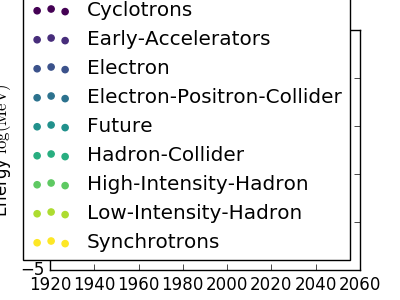
\includegraphics[scale=0.35]{acc_logE.png}\\
	\captionof{figure}{Shows the livingston plot for all accelerators found from the 1930's onward 
		grouped by the type of accelerator.}

	The same data was used to make a plot for newer detectors from the 1990's up to some future proposed detectors.
	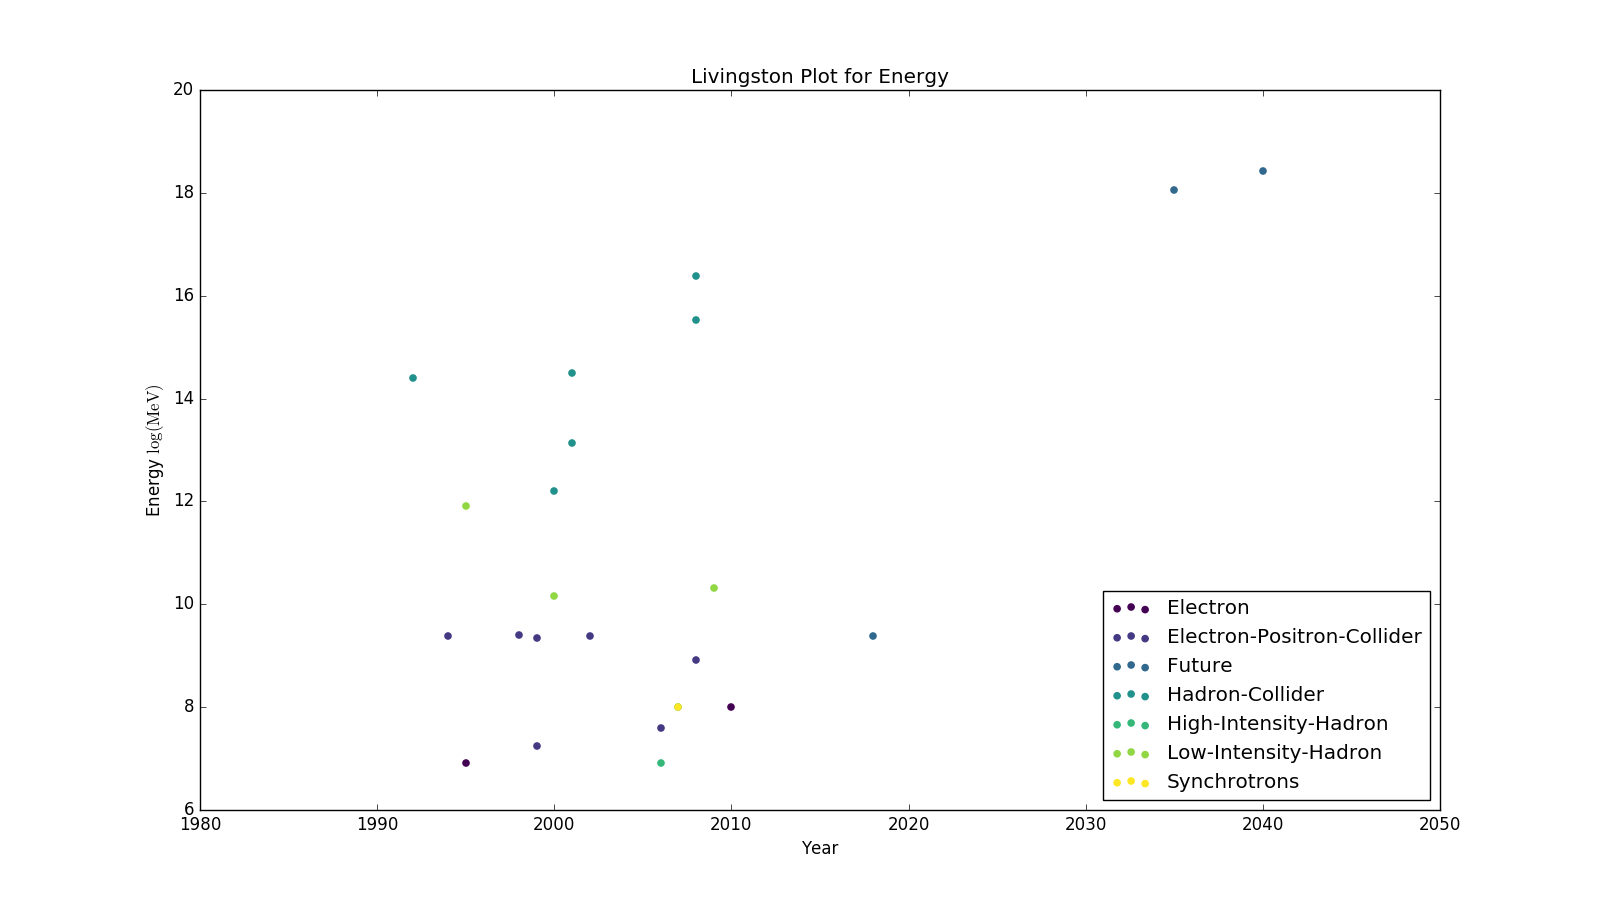
\includegraphics[scale=0.35]{acc_logE_90.png}\\
	\captionof{figure}{The same livingston plot but for accelerators after 1990.}

	\item Information on the luminosity was also found and placed into another plot.
	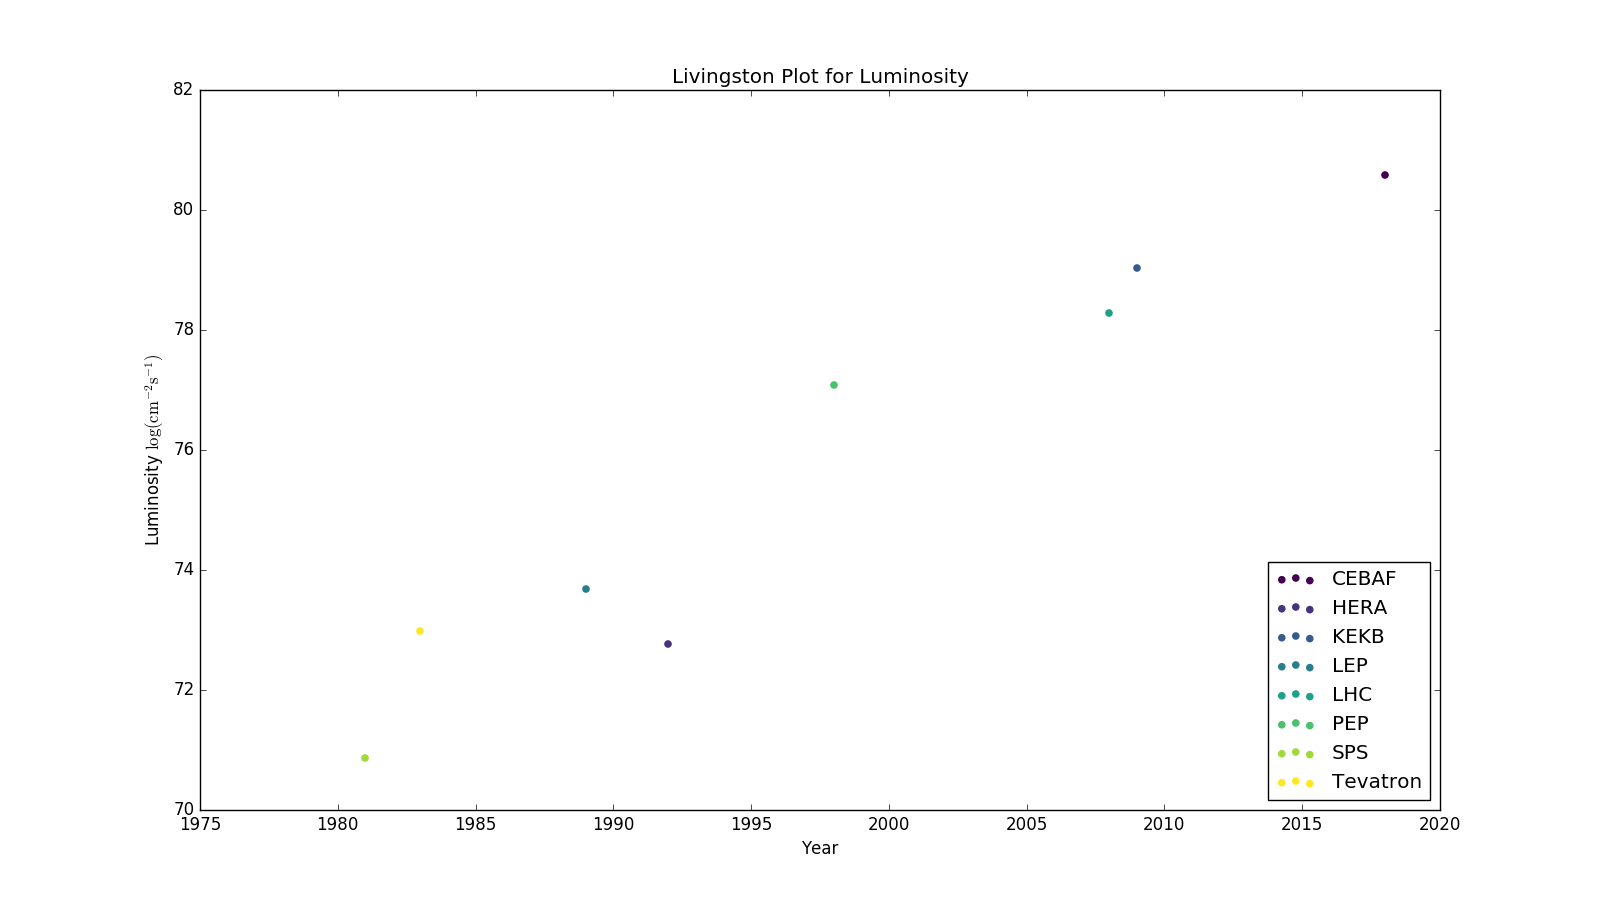
\includegraphics[scale=0.35]{acc_LogLum.png}\\
	\captionof{figure}{Shows the livingston plot for luminosity of some acceleartors.}




\end{enumerate}

\end{document}
